\documentclass[border=10pt]{standalone}

\usepackage{tikz}
\usepackage{tikzsymbols}
\usetikzlibrary{calc,patterns,shapes.geometric}

\def\centerarc[#1](#2)(#3:#4:#5){\draw[#1] ($(#2)+({#5*cos(#3)},{#5*sin(#3)})$) arc (#3:#4:#5);}

\begin{document}
	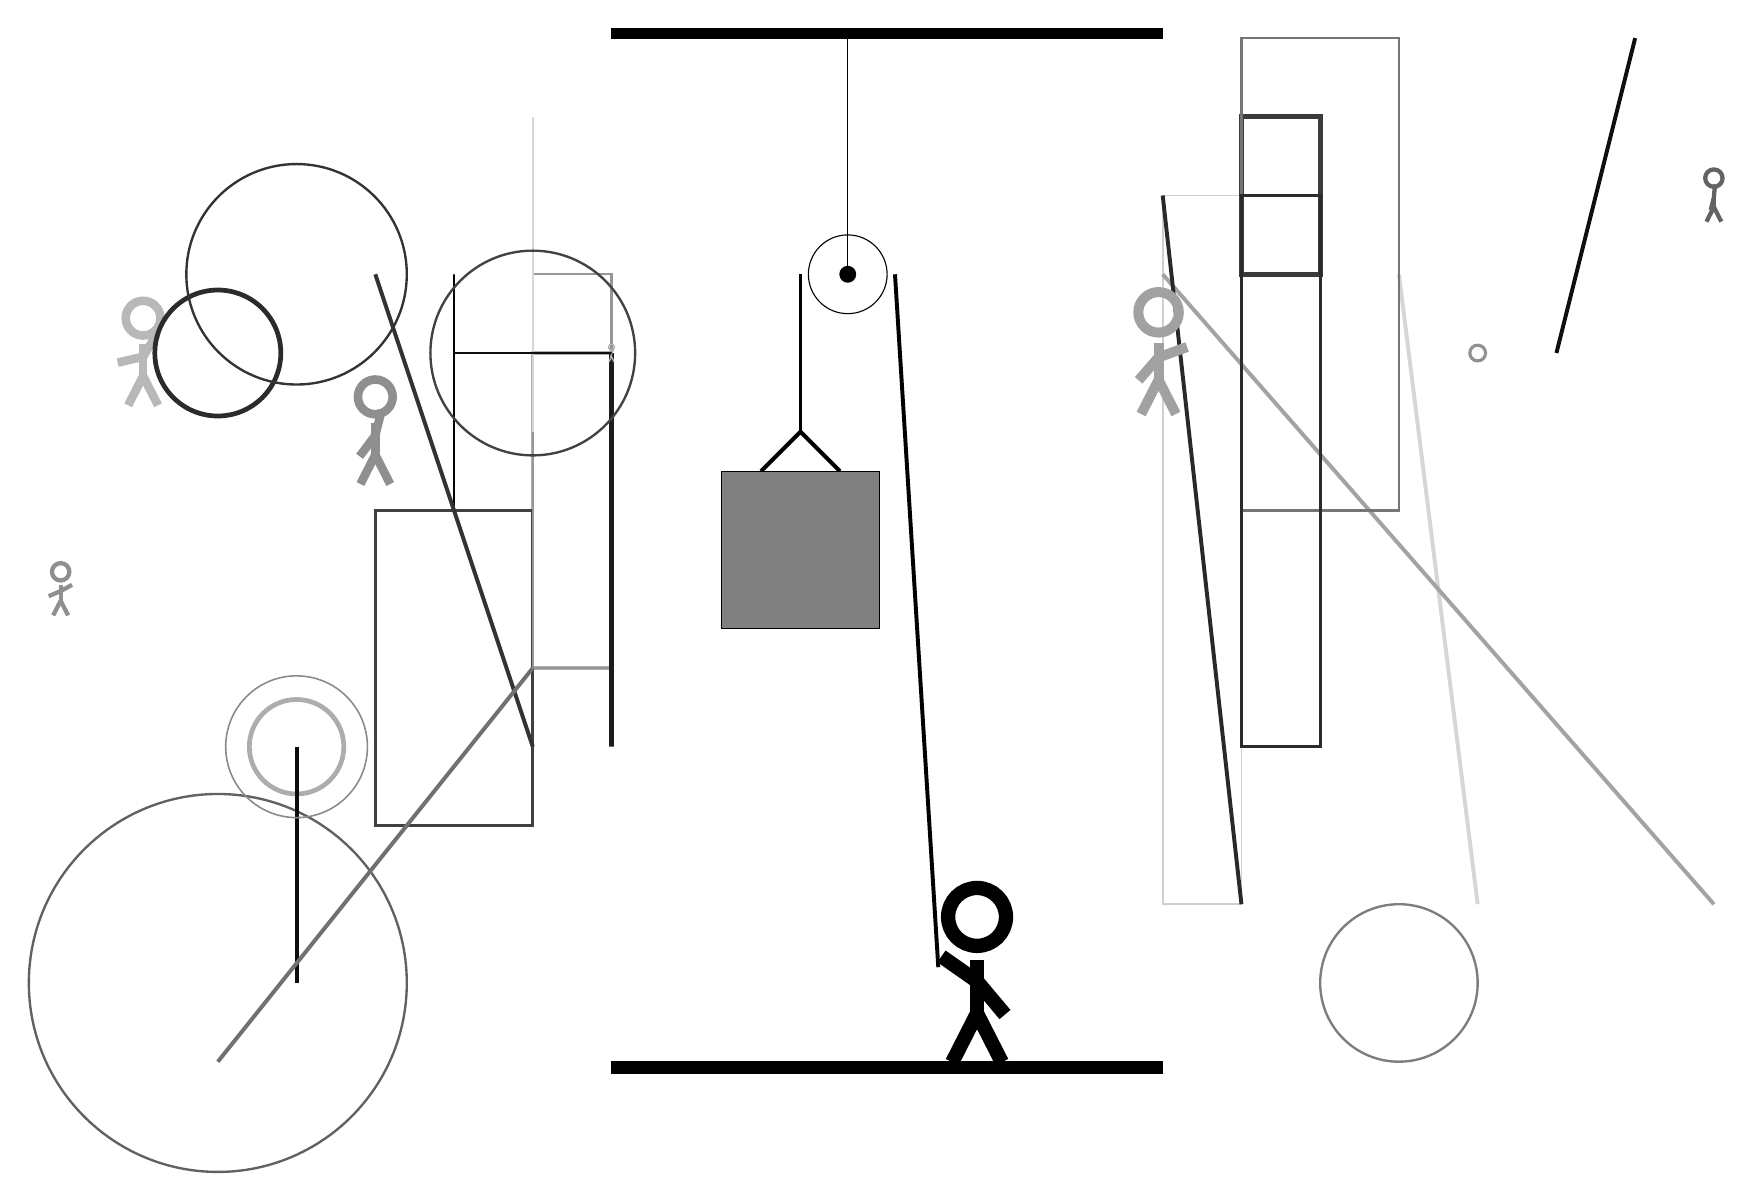
\begin{tikzpicture}
		%%%%% START %%%%%
		
		\draw[fill=black] (-2, 10) rectangle (5, 10.125);
		
		\draw (1, 7) circle (0.5);
		\draw[fill=black] (1, 7) circle (0.1);
		\draw (1, 10) -- (1, 7);
		
		\draw[line width=0.5mm] (-0.1, 4.5) -- (0.4, 5.0) -- (0.9, 4.5);
		\draw[fill=black!50] (-0.6, 4.5) rectangle (1.4, 2.5);
		
		\draw[line width=0.5mm] (0.4, 7) -- (0.4, 5.0);
		\centerarc[line width=0.5mm](1, 7)(0:180:0.6);
		\draw[line width=0.5mm](1.6, 7) -- (2.15, -1.8);
		
		\node at (2.6, -1.9) {\Strichmaxerl[10][-35][-50]};
		
		\draw[line width=0.4mm, color=black!32] (-2, 2) rectangle (-3, 6);
		
		\node[line width=0.6mm, color=black!28] at (-8, 6) {\Strichmaxerl[6][13][59]};
		\node[line width=0.7mm, color=black!44] at (-9, 3) {\Strichmaxerl[3][23][29]};
		\draw[line width=0.4mm, color=black!17] (6, 10) rectangle (6, 9);
		
		\draw[line width=0.4mm, color=black!75] (-3, 4) rectangle (-5, 0);
		
		\draw [line width=0.6mm, color=black!32](-6, 1) circle (0.6);
		
		\draw[line width=0.3mm, color=black!41] (-3, 7) rectangle (-2, 2);
		\draw[line width=0.5mm, color=black!16](9, -1) -- (8, 7);
		\draw [line width=0.3mm, color=black!62](-7, -2) circle (2.4);
		\draw[line width=0.2mm, color=black!19] (6, -1) rectangle (5, 8);
		\draw[line width=0.2mm, color=black!99] (-4, 4) rectangle (-4, 7);
		
		\draw[line width=0.5mm, color=black!36](5, 7) -- (12, -1);
		\draw[line width=0.5mm, color=black!95](-6, -2) -- (-6, 1);
		
		\draw[line width=0.6mm, color=black!89] (-2, 1) rectangle (-2, 6);
		\draw [line width=0.6mm, color=black!83](-7, 6) circle (0.8);
		\draw [line width=0.3mm, color=black!80](-6, 7) circle (1.4);
		\draw [line width=0.3mm, color=black!51](8, -2) circle (1.0);
		\draw[line width=0.6mm, color=black!77] (6, 7) rectangle (7, 9);
		\draw [line width=0.2mm, color=black!46](-6, 1) circle (0.9);
		\draw[line width=0.5mm, color=black!84](5, 8) -- (6, -1);
		\draw[line width=0.3mm, color=black!54] (6, 10) rectangle (8, 4);
		\draw[line width=0.4mm, color=black!83] (7, 1) rectangle (6, 8);
		
		\node[line width=0.3mm, color=black!31] at (-2, 6) {\Strichmaxerl[1][78][64]};
		\node[line width=0.5mm, color=black!37] at (5, 6) {\Strichmaxerl[7][49][20]};
		\draw[line width=0.5mm, color=black!94](10, 6) -- (11, 10);
		
		\draw[line width=0.5mm, color=black!80](-5, 7) -- (-3, 1);
		\node[line width=0.2mm, color=black!44] at (-5, 5) {\Strichmaxerl[6][53][76]};
		\draw[line width=0.5mm, color=black!56](-7, -3) -- (-3, 2);
		
		\node[line width=0.5mm, color=black!61] at (12, 8) {\Strichmaxerl[3][76][85]};
		
		\draw[line width=0.2mm, color=black!16] (-3, 5) rectangle (-3, 9);
		\draw [line width=0.4mm, color=black!43](9, 6) circle (0.1);
		
		\draw [line width=0.3mm, color=black!74](-3, 6) circle (1.3);
		\draw[line width=0.3mm, color=black!94] (-4, 6) rectangle (-2, 6);
		
		\draw[fill=black] (-2, -3) rectangle (5, -3.15);
		
		%%%%% END %%%%%
	\end{tikzpicture}
\end{document}